\let\lesson\undefined
\newcommand{\lesson}{\phantomlesson{Bài 21: Động học của chuyển động tròn.}}
\chapter[Động học của chuyển động tròn]{Động học của chuyển động tròn}
\setcounter{section}{0}
\section{Lý thuyết}
\subsection{Chuyển động tròn}
Chuyển động tròn là chuyển động có quỹ đạo là một đường tròn.\\
\textbf{\textit{Ví dụ:}} một điểm trên cánh quạt chuyển động theo một đường tròn khi cánh quạt quay, chuyển động của một vệ tinh nhân tạo xung quanh Trái Đất.
\begin{center}
	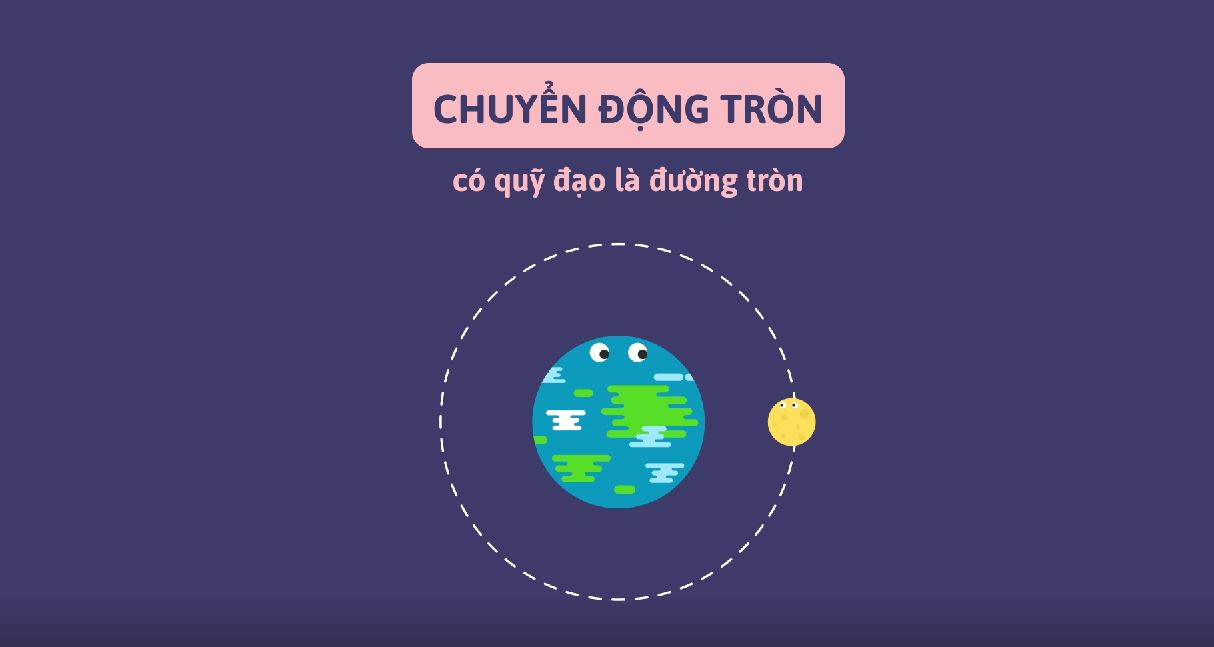
\includegraphics[scale=0.3]{../figs/VN10-PH-06-L-005-1-V2-01.jpg}
\end{center}
\subsection{Tốc độ trung bình trong chuyển động tròn}
 Tốc độ trung bình trong chuyển động tròn là độ dài cung tròn mà vật đi được trong một đơn vị thời gian.
\begin{center}
	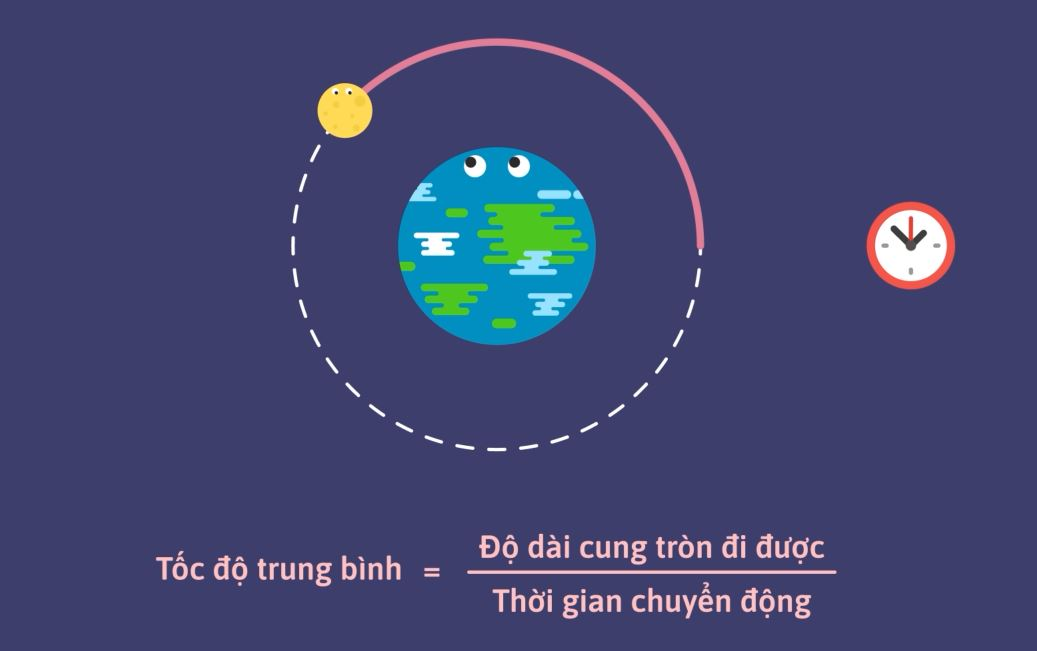
\includegraphics[scale=0.3]{../figs/VN10-PH-06-L-005-1-V2-02.jpg}
\end{center}
\subsection{Chuyển động tròn đều}
Chuyển động tròn đều là chuyển động có quỹ đạo tròn và có tốc độ trung bình không đổi trên mọi cung tròn của quỹ đạo. 

\begin{center}
	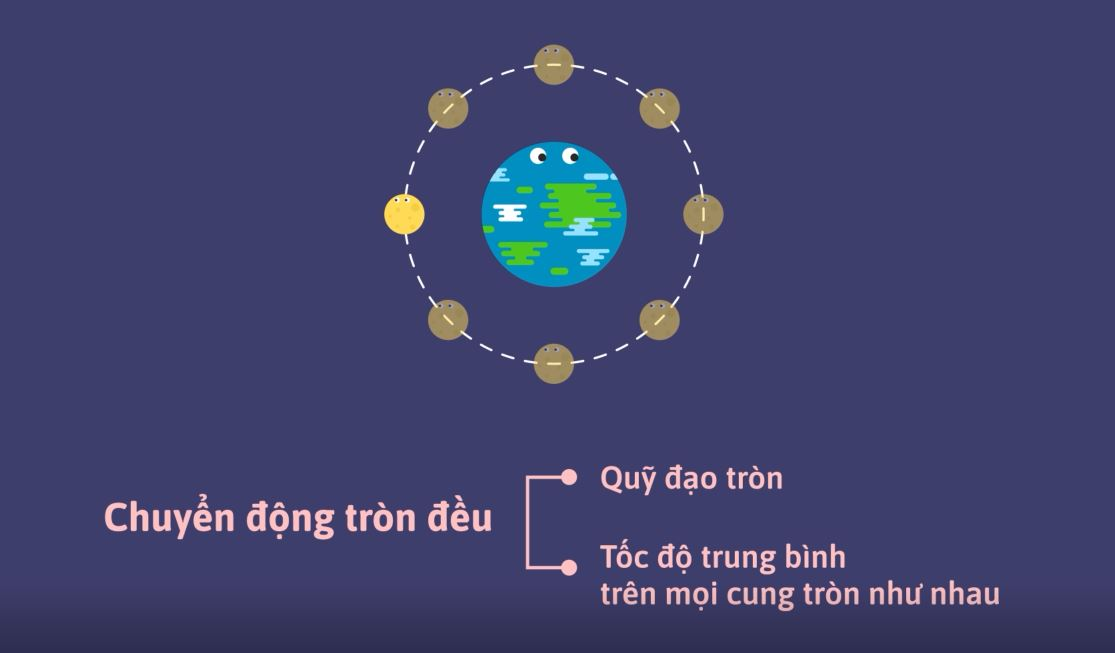
\includegraphics[scale=0.3]{../figs/VN10-PH-06-L-005-1-V2-03.jpg}
\end{center}
\subsection{Độ dịch chuyển góc}
Giả sử một vật chuyển động trên một đường tròn bán kính $r$. Trong thời gian $\Delta t$ vật đi được quãng đường $\Delta s$. Góc $\Delta \alpha$ ứng với cung tròn $\Delta s$ mà vật đã đi được kể từ vị trí ban đầu gọi là độ dịch chuyển góc:
$$\Delta \alpha = \dfrac{\Delta s}{r}$$

Đơn vị của độ dịch chuyển góc là rad.
\luuy{Trong Vật lí người ta thường đo góc theo đơn vị radian (kí hiệu rad), với $\SI{1}{rad}$ là số đo góc ở tâm một đường tròn chắn cung có độ dài bằng bán kính đường tròn đó.
	$$\SI{1}{rad} = \dfrac{180^\circ}{\pi} = \dfrac{180^\circ}{\SI{3.1416}{}\ldots} \approx\SI{57.2958}{^\circ}$$
	\begin{center}
		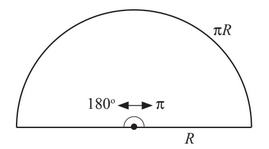
\includegraphics{../figs/G10-026-1}
	\end{center}
}
\subsection{Tốc độ góc và tốc độ dài trong chuyển động tròn}
\subsubsection{Tốc độ góc}
Tốc độ góc trong chuyển động tròn có giá trị bằng độ dịch chuyển góc trong một đơn vị thời gian:
$$\omega = \frac{\Delta \alpha}{\Delta t}$$

Đơn vị của tốc độ góc trong hệ đơn vị SI là $\SI{}{\radian/\second}$.\\

Trong chuyển động tròn đều, tốc độ góc của vật không đổi. 
\begin{center}
	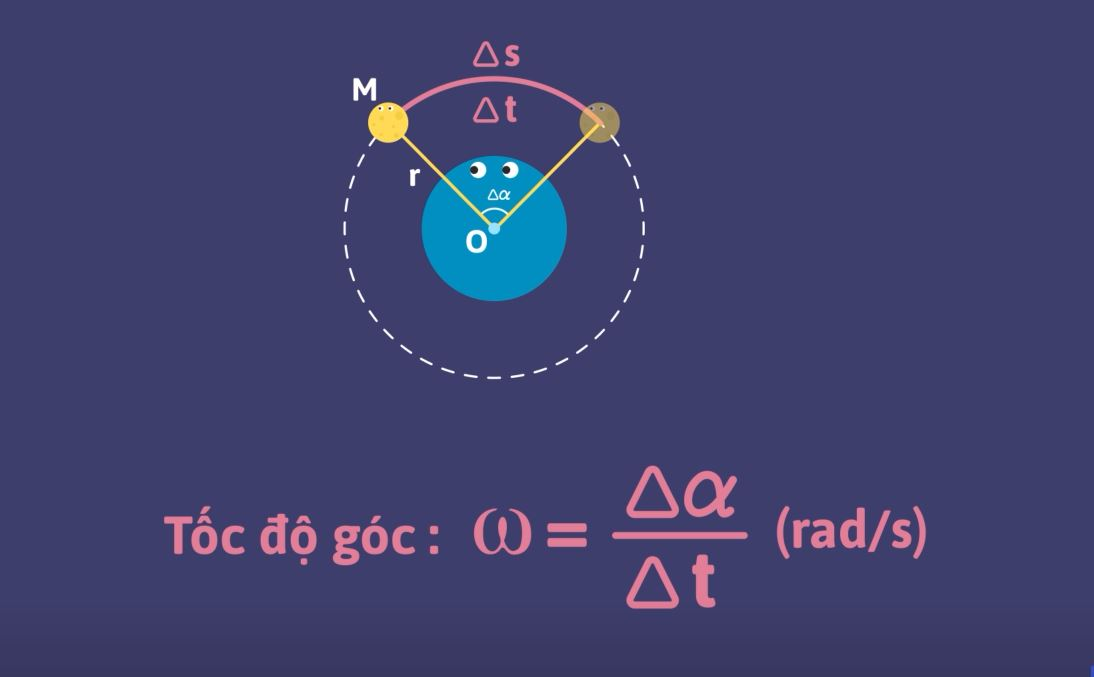
\includegraphics[scale=0.3]{../figs/VN10-PH-06-L-005-2-V2-02.jpg}
\end{center}
\subsubsection{Tốc độ dài}
Trong chuyển động tròn, mỗi điểm trên bán kính đều có cùng tốc độ góc, nhưng vì mỗi điểm này có thể có quãng đường chuyển động khác nhau nên để phân biệt với tốc độ góc, ta sử dụng khái niệm tốc độ dài.

Tốc độ dài (gọi tắt là là tốc độ) của một chất điểm chuyển động tròn được tính bằng quãng đường mà chất điểm di chuyển được trong một đơn vị thời gian:
$$v=\frac{\Delta s}{\Delta t} $$

Đơn vị của tốc độ dài trong hệ đơn vị SI là $\SI{}{\meter/\second.}$.\\

Trong chuyển động tròn đều, tốc độ dài của vật không đổi. \\
\begin{center}
	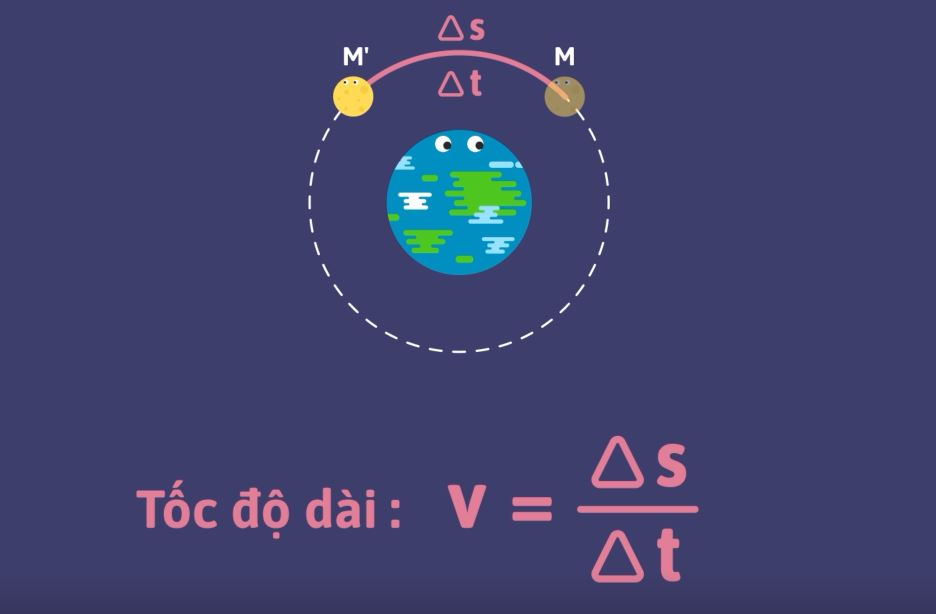
\includegraphics[scale=0.3]{../figs/VN10-PH-06-L-005-2-V2-01.jpg}
\end{center}	

\begin{minipage}{0.6\textwidth}
	Khi nói về phương, chiều của tốc độ dài, người ta sử dụng khái niệm vectơ vận tốc (gọi tắt là vận tốc). Vận tốc trong chuyển động tròn có phương tiếp tuyến với đường tròn quỹ đạo và có chiều là chiều của chuyển động.
	
	Trong chuyển động tròn đều, độ lớn của vận tốc tức thời không đổi nhưng hướng luôn thay đổi.
\end{minipage}
\begin{minipage}{0.4\textwidth}
	\begin{center}
		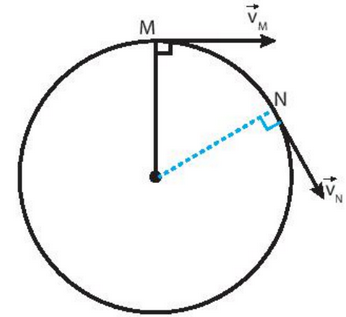
\includegraphics[scale=0.6]{../figs/G10-026-2}
	\end{center}
\end{minipage}


\subsubsection{Liên hệ giữa tốc độ góc và tốc độ dài}
Công thức liên hệ giữa tốc độ góc và tốc độ dài:
$$v=r\omega,$$ 
trong đó, $r$ là bán kính quỹ đạo tròn.		


\subsection{Chu kì và tần số}
Ngoài tốc độ, tốc độ góc, trong chuyển động tròn đều người ta còn quan tâm đến các đại lượng như chu kì và tần số.

\subsubsection{Chu kì}

Chu kì (kí hiệu là $T$) trong chuyển động tròn đều là thời gian để vật đi được một vòng tròn.

Đơn vị của chu kì trong hệ đơn vị SI là giây $\left(\si{\second}\right)$.

\subsubsection{Tần số}
Tần số (kí hiệu là $f$) là số vòng vật đi được trong một giây.

Đơn vị tần số là hertz (Hz).

\subsubsection{Liên hệ giữa chu kì, tần số, và tốc độ góc}

Công thức liên hệ giữa chu kì, tần số và tần số góc:

$$T=\dfrac{1}{f}=\dfrac{2\pi}{\omega},$$
trong đó, $T$ là chu kì, $f$ là tần số, $\omega$ là tốc độ góc. 				

\subsection{Gia tốc hướng tâm}
\begin{center}
	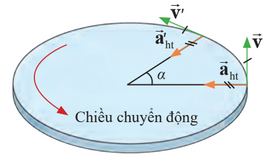
\includegraphics[scale=1]{../figs/G10-027-1}
	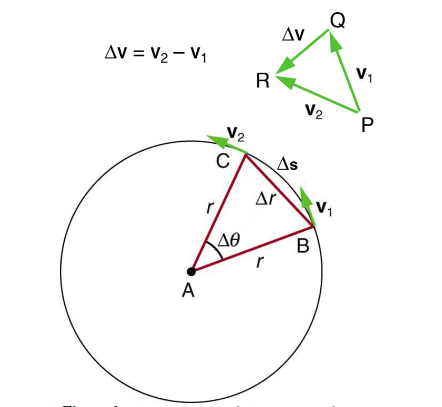
\includegraphics[height=5cm]{../figs/G10-027-1b}
\end{center}

\begin{itemize}
	\item Trong chuyển động tròn đều, vectơ gia tốc $\vec{a}=\frac{\Delta\vec{v}}{\Delta t}$  hướng vào  tâm đường tròn.
	\item Vectơ gia tốc hướng tâm đặc trưng cho sự biến đổi của vectơ vận tốc, kí hiệu là $\vec{a}_{ht}$.
	\item Độ lớn của vectơ gia tốc hướng tâm:
	\begin{equation*}
		a_\text{ht}=\frac{v^2}{r}=\omega^2 \cdot r.
	\end{equation*}
\end{itemize}
\section{Mục tiêu bài học - Ví dụ minh họa}
\begin{dang}{Nhận biết đặc điểm của  chuyển động tròn đều}
	\viduii{1}{Chuyển động nào dưới đây là chuyển động tròn đều?
		\begin{mcq}
			\item Chuyển động của mắt xích xe đạp khi xe chạy.
			\item Chuyển động của đầu cánh quạt trần khi quay ổn định.
			\item Chuyển động của đầu cánh quạt trần khi vừa bật.
			\item Chuyển động của con lắc đồng hồ.
		\end{mcq}
	}
	{	\begin{center}
			\textbf{Hướng dẫn giải}
		\end{center}
		
		Chuyển động tròn đều là chuyển động có các đặc điểm:
		\begin{itemize}
			\item Quỹ đạo là một đường tròn;
			\item Tốc độ trung bình trên mọi cung tròn là như nhau.
		\end{itemize}
		Chuyển động A không thỏa điều kiện quỹ đạo tròn. Chuyển động C, khi vừa bật quạt thì tốc độ quay của đầu cánh quạt tăng dần. Chuyển động D không thỏa điều kiện tốc độ trung bình như nhau trên mọi cung tròn. Chuyển động B thỏa mãn cả hai điều kiện. 
		
		\textbf{Đáp án: B}.
		
	}
	\viduii{1}
	{Chuyển động nào sau đây có thể xem như là chuyển động tròn đều?
	\begin{mcq}
		\item Chuyển động của một vật được ném xiên từ mặt đất.
		\item Chuyển động trong mặt phẳng thẳng đứng của một vật được buộc vào một dây có chiều dài cố định.
		\item Chuyển động của một vệ tinh nhân tạo có vị trí tương đối không đổi với một điểm trên mặt đất (vệ tinh địa tĩnh).
		\item Chuyển động của một quả táo khi rời ra khỏi cành cây.
	\end{mcq}
}
{\begin{center}
		\textbf{Hướng dẫn giải}
	\end{center}
Chuyển động tròn đều cần thoả 2 điều kiện:
\begin{itemize}
	\item Quỹ đạo chuyển động là đường tròn.
	\item Tốc độ trung bình như nhau trên mọi cung tròn.
\end{itemize}
Chuyển động của một vật được ném xiên từ mặt đất có quỹ đạo là parabol.

Chuyển động trong mặt phẳng thẳng đứng của một vật được buộc vào một dây có chiều dài cố định chưa hẳn là chuyển động tròn đều vì chưa mô tả rõ trạng thái chuyển động của vật.

Chuyển động của một quả táo khi rời ra khỏi cành cây là chuyển động thẳng biến đổi.

Chuyển động của một vệ tinh nhân tạo có vị trí tương đối không đổi đối với một điểm trên mặt đất (vệ tinh địa tĩnh) là chuyển động tròn đều.

\textbf{Đáp án C.}


}
	
\end{dang}
\begin{dang}{Biểu diễn đơn vị độ dịch chuyển góc}
	\viduii{2}{Đổi các góc sau từ độ sang radian: $30^\circ$, $90^\circ$.
	}
	{	\begin{center}
			\textbf{Hướng dẫn giải}
		\end{center}
		
		Ta có:
		$$x^\circ \longrightarrow \dfrac{x \pi}{180}\ \text{rad}.$$
		
		Đổi $$30^\circ \longrightarrow \dfrac{30\pi}{180}\ \text{rad} = \dfrac{\pi}{6}\ \text{rad}$$
		
		Đổi $$90^\circ \longrightarrow \dfrac{\SI{90}{\degree}\pi}{\SI{180}{\degree}}\ \text{rad} = \dfrac{\pi}{2}\ \text{rad}$$
		
		\begin{center}
			\textbf{Câu hỏi tương tự}
		\end{center}
		
		Đổi các góc sau từ độ sang radian: $105^\circ$, $120^\circ$, $270^\circ$.
		
		\textbf{Đáp án:} $105^\circ \longrightarrow \dfrac{7\pi}{12}\ \text{rad}$; $120^\circ \longrightarrow \dfrac{2\pi}{3}\ \text{rad}$; $270^\circ \longrightarrow \dfrac{3\pi}{22}\ \text{rad}$.
	}
	\viduii{2}{Đổi các góc sau từ radian sang độ: $\SI{0.25}{rad}$, $\SI{0.5}{rad}$.
	}
	{	\begin{center}
			\textbf{Hướng dẫn giải}
		\end{center}
		
		Ta có:
		$$x\ \text{rad} \longrightarrow \left(\dfrac{x \cdot 180}{\pi}\right)^\circ.$$
		
		Đổi $$\SI{0.25}{rad} \longrightarrow \dfrac{0,25 \cdot \SI{180}{\degree}}{\pi} = 14,33^\circ$$
		
		Đổi $$\SI{0.5}{rad} \longrightarrow \dfrac{0,5 \cdot \SI{180}{\degree}}{\pi} = 28,66^\circ$$
		
		\begin{center}
			\textbf{Câu hỏi tương tự}
		\end{center}
		
		Đổi các góc sau từ radian sang độ: $\xsi{0,5\pi}{rad}$, $\xsi{\pi}{rad}$.
		
		\textbf{Đáp án:} $\xsi{0,5\pi}{rad} \longrightarrow 90^\circ$; $\xsi{\pi}{rad} \longrightarrow 180^\circ$.
	}
\end{dang}
\begin{dang}{Tính tốc độ dài, tốc độ góc, chu kỳ, tần số trong chuyển động tròn đều}
	\viduii{2}{Một vệ tinh nhân tạo bay quanh Trái Đất theo một quỹ đạo tròn. Chu kì của vệ tinh là $88\ \text{phút}$. Tính tốc độ góc của vệ tinh. 
	}
	{	\begin{center}
			\textbf{Hướng dẫn giải}
		\end{center}
		Tốc độ góc của vệ tinh:
		$$T=\frac{2\pi}{\omega} \quad\Rightarrow\quad \omega = \frac{\pi}{2640}\ \text{rad/s}.$$ 
		
		\begin{center}
			\textbf{Câu hỏi tương tự}
		\end{center}
		
		Roto trong một tổ máy của nhà máy thủy điện Hòa Bình quay 125 vòng mỗi phút. Hãy tính tốc độ góc của roto này theo đơn vị rad/s.
		
		\textbf{Đáp án:} $\omega \approx \SI{13.1}{rad/s}$.
	}
	
	\viduii{3}{
		Kim phút của đồng hồ dài gấp 1,5 lần kim giờ. Hỏi tốc độ dài của đầu kim phút lớn gấp mấy lần tốc độ dài của đầu kim giờ?
	}
	{	\begin{center}
			\textbf{Hướng dẫn giải}
		\end{center}
		
		Gọi: 
		\begin{itemize}
			\item  $R_1$, $R_2$ lần lượt là chiều dài kim phút và kim giờ
			$$\dfrac{R_1}{R_2}=1,5;$$
			\item $\omega_1, \omega_2$ lần lượt là tốc độ góc của kim phút và kim giờ. Kim phút quay một vòng ($2\pi\ \SI{}{\radian}$) trong 1 giờ, kim giờ quay một vòng trong 12 giờ, do đó 
			$$
			\dfrac{\omega_1}{\omega_2}=12
			$$
		\end{itemize}
		
		
		Ta lập được tỉ số: $$\dfrac{v_1}{v_2}=\dfrac{\omega_1 \cdot R_1}{\omega_2 \cdot R_2}=\dfrac{\omega_1}{\omega_2}\cdot\dfrac{R_1}{R_2}=18.$$
		
		\begin{center}
			\textbf{Câu hỏi tương tự}
		\end{center}
		
		Biết chiều dài kim phút và kim giây của một chiếc đồng hồ lần lượt là $\SI{4}{cm}$ và $\SI{5}{cm}$. Hãy tính:
		\begin{enumerate}[label=\alph*)]
			\item Tỉ số chu kì quay của hai kim.
			\item Tỉ số tốc độ dài của đầu kim phút và đầu kim giây.
		\end{enumerate}
		
		\textbf{Đáp án:}
		\begin{enumerate}[label=\alph*)]
			\item $\frac{T_\text{phút}}{T_\text{giây}}=60$.
			\item $\frac{v_\text{phút}}{v_\text{giây}}=\dfrac{1}{75}$.
		\end{enumerate}
	}
	
	
	
\end{dang}
\begin{dang}{Tính gia tốc hướng tâm trong chuyển động tròn đều}
	
	\viduii{2}{Một vệ tinh nhân tạo ở độ cao $250\ \text{km}$ bay quanh Trái Đất theo một quỹ đạo tròn. Chu kì của vệ tinh là $88\ \text{phút}$. Tính gia tốc hướng tâm của vệ tinh. Cho bán kính Trái Đất là $6400\ \text{km}$
	}
	{	\begin{center}
			\textbf{Hướng dẫn giải}
		\end{center}
		
		Khoảng cách từ vệ tinh đến tâm Trái Đất: 
		$$r=250\ \text{km}+6400\ \text{km} =6650\ \text{km}=6650000\ \text{m}. $$
		Tốc độ góc của vệ tinh:
		$$T=\frac{2\pi}{\omega} \Rightarrow \omega = \frac{\pi}{2640}\ \text{rad/s}.$$ 
		Gia tốc hướng tâm của vệ tinh: 
		
		$$a_{ht}=\omega^2 \cdot r \approx \SI{9,41}{ \meter/\second^2}.$$ 
		
	}
	
	\viduii{2}{Một vật chuyển động theo đường tròn bán kính $r = \SI{100}{cm}$ với gia tốc hướng tâm $a_\text{ht} = \SI{4}{cm/s}^2$. Tính chu kì của chuyển động.
		
	}
	{	\begin{center}
			\textbf{Hướng dẫn giải}
		\end{center}
		
		Tốc độ dài của chuyển động
		$$a_\text{ht} =\dfrac{v^2}{r} \Rightarrow v =\sqrt {ra_\text{ht}}.$$
		
		Chu kì của chuyển động là
		$$T =\dfrac{2\pi}{\omega} = \dfrac{2\pi r}{v} = 2\pi \sqrt{\dfrac{r}{a_\text{ht}}} \approx \SI{31.415}{\second}.$$
		
	}
\end{dang}